\section{ROS}
ROS(Robot Operating System)は, ロボット開発を効率化するためのオープンソースソフトウェアフレームワークである. 
複数のプログラミング言語向けのライブラリや, センサや状態を可視化するツール群, ノード間のメッセージ通信機構, およびパッケージによるモジュール管理機能を備えている点が特徴である. 
ROSにおける基本的な実行単位はノードであり, ノードはトピックやサービスといった仕組みを通じて情報を交換する. 
これにより, センサデータの取得や制御アルゴリズム, 経路計画などを個別のモジュールとして構成し, 分散して動作させることが可能となる. 
さらに, 既成のアルゴリズムやデバイス向けソフトウェアをパッケージとして利用することで, 開発者は低コストかつ短期間で複雑な機能を実装することができる. 



\section{ナビゲーション}
ROS Navigation stack\cite{navstack}は, 自律移動ロボットが環境内を自律的に移動するためのソフトウェアフレームワークである. 主に以下の要素から構成されている. 
\begin{itemize}
     \item \textbf{自己位置推定}\\
     ロボットは地図上で自己位置を推定する必要がある. その代表的な手法として, AMCL(Adaptive Monte Carlo Localization)が用いられる. 
     AMCLはROS Navigation Stackで自己位置推定を行う確率的アルゴリズムであり, LiDARやオドメトリ情報をもとに多数の仮説(パーティクル)を生成し, 
     それぞれの重みを更新することでロボットの位置を推定する. また, 状況に応じてパーティクル数を動的に調整することで精度と計算負荷のバランスを取る特徴をもつ. 
     一方で, その性能はオドメトリ誤差やレーザノイズなど多くのパラメータ設定に依存しており, 実環境に応じたチューニングが重要となる. 
     \figref{Fig:lamcl_example}に自己位置推定の様子を示す. 
     \begin{figure}[hbtp]
     \centering
          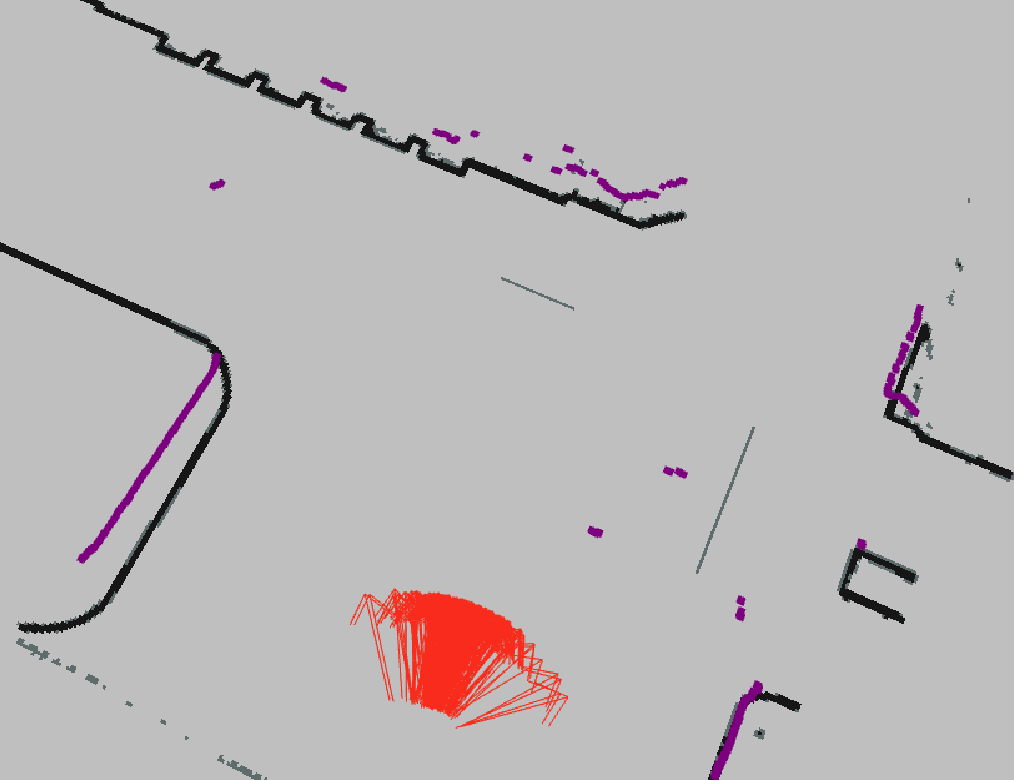
\includegraphics[keepaspectratio, scale=0.2]
           {images/amcl_example.png}
          \caption{Localization in Rviz}
          \label{Fig:lamcl_example}
     \end{figure}

     \item \textbf{地図生成}\\
     未知領域においては, 環境のマッピングのため, SLAM(Simultaneous Localization and Mapping)が必要となる. 
     SLAMは, ロボットが未知の環境内で自己位置を推定しながら同時に地図を生成するための手法であり, 
     自律移動の基盤技術の一つである. ロボットはLiDARやカメラなどのセンサ情報を取得し, 環境内の特徴点や障害物を検出することで地図を構築すると同時に, 
     自身の位置をその地図上で推定する. この相互依存的な推定を繰り返すことで, 外部基準を持たない環境でも自己位置と地図を同時に確立できる. 
     \figref{Fig:Map}にSLAMで作成された地図を示す. 
     \begin{figure}[hbtp]
     \centering
          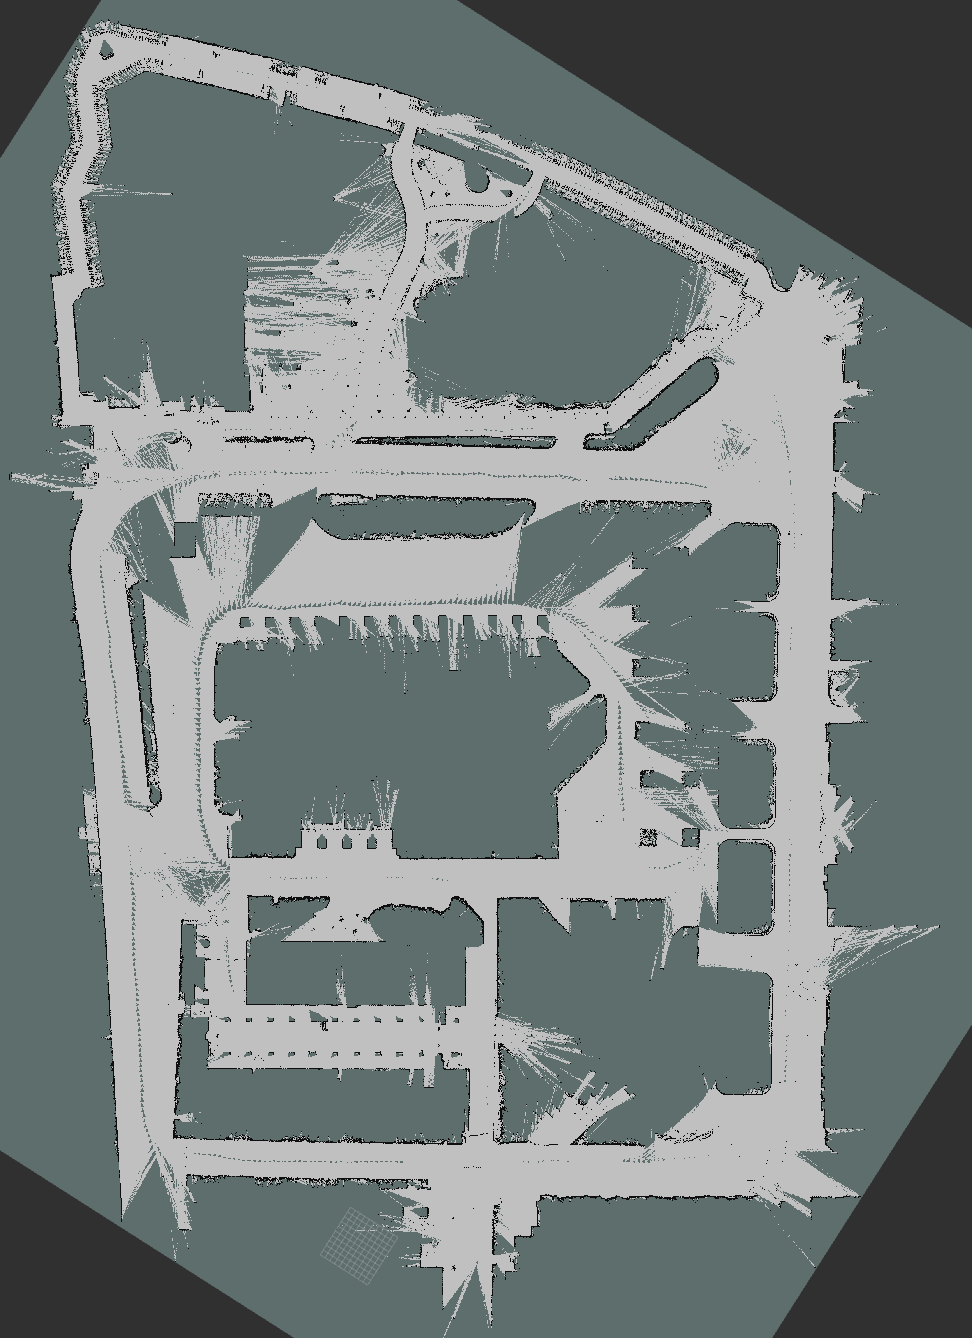
\includegraphics[keepaspectratio, scale=0.25]
           {images/slam_toolbox.png}
          \caption{Map created with SLAM}
          \label{Fig:Map}
     \end{figure}

     \item \textbf{経路計画}\\
     経路計画は, ロボットが目的地へ到達するための経路を生成, 追従するプロセスであり, ナビゲーションシステムの中心的な役割を担う. 
     大域的経路計画は, 静的な地図情報をもとに, ロボットの現在位置から目的地までの全体的な経路を計算する段階である. 
     ここでは主にDijkstra法やA*アルゴリズムといったグラフ探索手法が用いられ, 障害物を避けつつコストマップ上で最短または最適な経路を算出する. 
     一方, 局所的経路計画は, ロボットが実際に移動する際の動作をリアルタイムに制御する段階であり, 
     センサ情報をもとに動的な障害物を回避しながら経路を追従する. 
     代表的な手法であるDWA(Dynamic Window Approach)は, ロボットの運動学的制約を考慮しつつ, 
     速度空間内で安全かつ効率的な制御コマンドを探索するアルゴリズムである. 
     DWAは目標方向の進行性, 障害物との距離, 安全性など複数の評価関数を組み合わせて最適な行動を選択することで, 
     滑らかな走行と衝突回避を両立させている. 
     \item \textbf{コストマップ}\\
     コストマップは, ロボットの経路計画において基盤となる情報構造であり, 環境内の障害物や走行困難な領域を数値化して表現することで, 
     経路計画アルゴリズムが安全かつ効率的に移動できるようにする. 
     ROS Navigation stackでは, コストマップは, 静的マップと動的マップにに分けて管理される. 
     静的マップはあらかじめ生成された地図に基づく固定的な障害物情報を提供し, 
     局所的な経路計画や障害物回避の基盤として利用される. 
     一方, 動的マップはLiDARやカメラなどのセンサ情報をもとにリアルタイムで更新され, 
     移動中に出現する人などの動的障害物を反映する. コストマップ上では, 
     障害物が存在するセルの値が高く, 通行可能な領域は低い値で表現される. 
     この数値は経路計画アルゴリズムによって考慮され, ロボットはより安全でコストの低い経路を優先して移動する. 
     これにより, 経路計画は単に障害物を避けるだけでなく, 走行中の安全性を確保しつつ目標地点まで到達できるようになる. 
     \figref{Fig:costmap}にコストマップの一例を示す. 
     \begin{figure}[hbtp]
     \centering
          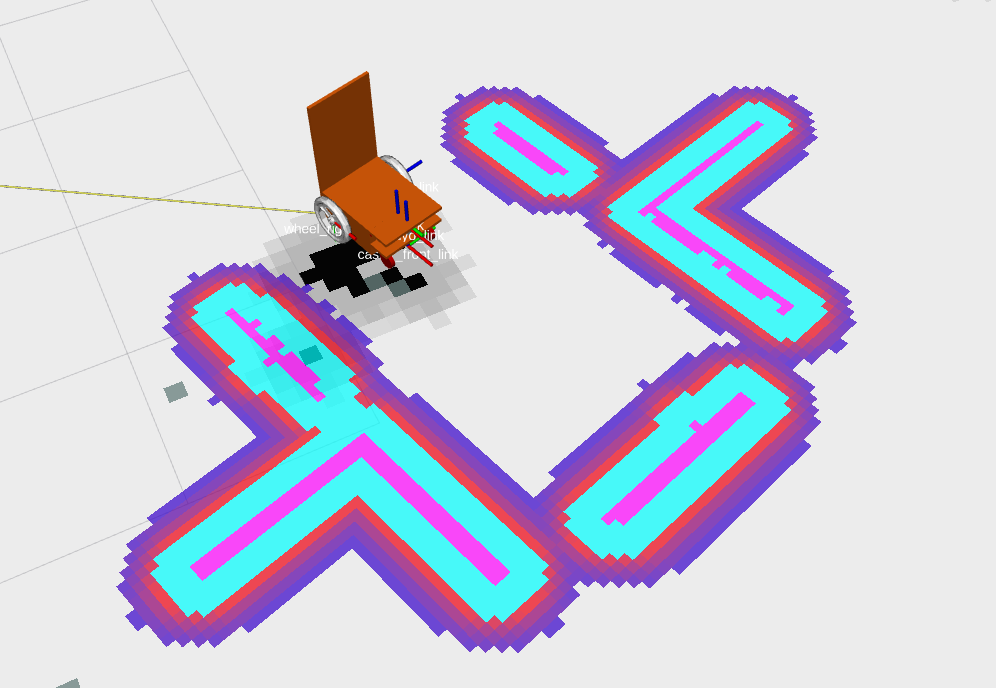
\includegraphics[keepaspectratio, scale=0.2]
           {images/costmap.png}
          \caption{Costmap in Rviz}
          \label{Fig:costmap}
     \end{figure}     
\end{itemize}